\documentclass[fleqn,10pt]{wlscirep}
\usepackage[utf8]{inputenc}
\usepackage[T1]{fontenc}
\usepackage{caption}
\usepackage[position=top]{subcaption}
\usepackage[export]{adjustbox}
\usepackage{array}

\newcommand{\si}[2]{$\mathrm{#1\,#2}$}

\title{Scientific Reports Title to see here}

\author[1,*]{Benjamin Lotter}
\author[1]{Srumika Konde}
\author[1]{Lam Vien Che}
\author[1]{Johnny Nguyen}
\author[1]{Lorenz Maximillian Schneider}
\author[2]{Michael Grau}
\author[1]{Martin Koch}
\author[1]{Peter Lenz}
\affil[1]{Philipps University of Marburg, Department of Physics, Marburg, 35032, Germany}
\affil[2]{University of Münster, Translationale Onkologie, Münster, 48149, Germany}
\affil[*]{corresponding.author@email.example}

%\keywords{Keyword1, Keyword2, Keyword3}

\begin{abstract}
Example Abstract. Abstract must not include subheadings or citations. Example Abstract. Abstract must not include subheadings or citations. Example Abstract. Abstract must not include subheadings or citations. Example Abstract. Abstract must not include subheadings or citations. Example Abstract. Abstract must not include subheadings or citations. Example Abstract. Abstract must not include subheadings or citations. Example Abstract. Abstract must not include subheadings or citations. Example Abstract. Abstract must not include subheadings or citations.
\end{abstract}
\begin{document}

\flushbottom
\maketitle
% * <john.hammersley@gmail.com> 2015-02-09T12:07:31.197Z:
%
%  Click the title above to edit the author information and abstract
%
\thispagestyle{empty}

\noindent Please note: Abbreviations should be introduced at the first mention in the main text – no abbreviations lists. Suggested structure of main text (not enforced) is provided below.

\section*{Introduction}
<<<<<<< .merge_file_a11164
Our planet is drowning in plastic litter that finds its way into our food and body over time.
=======
Our planet is drowning in plastic litter that can sneakily enter our body over time.
>>>>>>> .merge_file_a04972
An estimation showed that in 2010 at least 4.8 million tons of plastic litter has already entered our ocean\cite{Jambeck2015a}; a volume that will increase without an effective waste management plan\cite{Jambeck2015a, Geyer2017}. 
Once in the wild, plastic can persist for decades as most types are resistant to natural degradation processes\cite{Chamas2020}.
Environmental influences, however, can cause it to disintegrate into micron-sized particles commonly known as microplastics\cite{Thompson2004, Julienne2019, Zhang2021, Song2017, Duis2016}.
Almost invisible to the eye, they have now been detected on nearly every corner of our planet\cite{Duis2016,Chiba2018,Napper2020,Eerkes-Medrano2015,Andrady2011,Allen2019a}, in animals \cite{Barboza2020,Haave2021, Jamieson2019} and even in our food\cite{Koelmans2019,Zhang2020a}.
Since 2021, we also have the first evidence that microplastics are present in humans, when Ragusa et al. detected microplastics in the human placenta\cite{Ragusa2021}.

Plastic litter is highly diverse due to environmental influences and the sheer endless possibilities to produce plastic with desired material properties.
Therefore, to evaluate their detrimental effects on animals and humans, we need a deeper insight on the samples origins\cite{Prata2020, Campanale2020, Lim2021}.
Here, tools to detect and classify plastic litter at different stages play an indispensable role.
Studies on plastic pollution commonly use Raman and Fourier transform infrared (FTIR) spectroscopy solutions to analyse plastic samples\cite{Prata2019,Loder2015,Sun2019,Zhang2020b}.
<<<<<<< .merge_file_a11164
Both techniques, however, come with physical limitations\cite{Araujo2018a, Loder2015,Xu2019} and hence, some plastic litter types remain undetected to date.

Most recently, Ornik et al. \cite{Ornik2020} used photoluminescence (PL) spectroscopy for plastic identification.
By comparing spectral intensity ratios between different samples, they sucessfully distinguished plastics from non-plastic samples from the riverine and marine environment.
Such an identification method, however, may not be reproducible since measurements depend on different experimental factors such as hardware alignments, sample sites or even scientific experiences.
On the other hand, it is impractical to capture and quantify these influences as it is impossible to account for all possible factors.
Nevertheless, it raises the question if there are subsets in the spectra that can be used for the identification while being robust against such experimental variations.
=======
Both techniques, however, come with physical limitations\cite{Araujo2018a, Loder2015,Xu2019} and hence, we only cover a subset of plastic waste types out there.

Most recently, Ornik et al. \cite{Ornik2020} used photoluminescence (PL) spectroscopy for plastic identification.
By comparing the intensity ratios in the PL spectrum of different samples, they sucessfully distinguished plastics from non-plastic samples in the riverine and marine environment.
Such an identification method, however, may not be reproducible since a measurement can change with different experimental factors such as hardware alignments, sample sites or even scientific experiences.
On the other hand, it is impractical to capture and quantify these influences since it is impossible to account for all possible factors.
Nevertheless, it raises the question if there are subsets in the spectra that can be used for the identification while being robust against experimental variations.
>>>>>>> .merge_file_a04972
One possible solution is to capture a part of these variations and integrate them in a spectral library.
Once implemented, algorithms and mathematical models help unraveling the origins of the plastic sample.

For predictions that account for data variations, machine learning (ML) models are suitable candidates.
To generate a plastic waste prediction model, we apply a selected learning method on the labeled spectral dataset.
The model's performance partially depends on the number of input variables in a dataset, which, in our case, is the measured intensity for each channel of our spectrometer.
To improve the performance, it is common practice to reduce the number of variables while retaining the essential data information \cite{Aggarwal2001,Fodor2002}.
The efficiency to capture most of the information depends on the selected transformation technique.
Here, recently published technique termed as signal dissection by correlation maximization (SDCM) stands out which successfully discovered new hidden signatures in a gene expression dataset \cite{Grau2019}.
This is particularly attractive for PL-based plastic litter detection as it can identify type specific subspectra that are robust against experimental variations.

In this report, we demonstrate that SDCM is suitable to generate robust PL-based plastic litter identification models.
To demonstrate this, we look at two sets of ML models that are either based on a SDCM-transformed PL dataset or an untransformed dataset.
By comparing model's accuracies, i.e. the probability that a model based prediction is correct, we find consistently higher values for SDCM-based ML models than their counterparts.
This underlines the robustness of SDCM-transformed PL datasets against experimental variations.

\section*{Results}

\subsection*{Evaluation of ML models}
\begin{figure}[ht]
	\centering
	\begin{subfigure}[t]{0.45\textwidth}
		\includegraphics[valign=t]{figures/learningMethodVsaccuracy.pdf}
		\caption{Accuracy}
		\label{fig:learnMethodAccuracy}
	\end{subfigure}
	\hfill
	\begin{subfigure}[t]{0.45\textwidth}
		\includegraphics[valign=t]{figures/learningMethodVsf1.pdf}
		\caption{f1}
		\label{fig:learnMethodF1}
	\end{subfigure}
	\caption{Plot of the performance metrics \textit{accuracy} and \textit{f1} for different plastic classification models.}
\end{figure}

We evaluate the performance of SDCM-based classification models, by calculating the metrics \textit{accuracy} and \textit{f1} for all ML models.
Figures~\ref{fig:learnMethodAccuracy} and \ref{fig:learnMethodF1} show plots of the calculated values for accuracy and f1, respectively.
The models generated with the SVC and the Random Forest algorithm achieve performance metric values over \si{90}{\%} for all dimension reduction techniques.
In comparison to these two model types, the performance drops by \si{20}{\%} for models generated the Naive Bayes algorithm.
Thus, for plastic classification the former two methods are likely to be more suitable in the future.


\begin{figure}[ht]
	\centering
	\includegraphics[width=\textwidth]{figures/confusionMatrix.png}
	\caption{Confusion matrix for individual sample classes}
	\label{fig:confusionMatrix}
\end{figure}

\subsection*{Subsection}

Example text under a subsection. Bulleted lists may be used where appropriate, e.g.

\begin{itemize}
\item First item
\item Second item
\end{itemize}

\subsubsection*{Third-level section}
 
Topical subheadings are allowed.

\section*{Discussion}

The Discussion should be succinct and must not contain subheadings.

\section*{Methods}
\newcommand{\si}[2]{$\mathrm{#1\,#2}$}
\subsection*{Experimental setup}
\begin{figure}[ht]
	\centering
	\includegraphics{figures/experimentalSetup.png}
	\caption{Diagram of the photoluminescence spectroscopy setup.}
	\label{fig:experimentalSetup}
\end{figure}

\ref{fig:experimentalSetup} illustrates our experimental setup which we use to acquire the photoluminescence spectra. 
The beam path to excite the sample and induce photoluminescence emission is highlighted in blue.
For the excitation, we use a beam with a central wavelength of \si{405}{nm}.
This is achieved by using a laser that generates a beam with a central wavelength of \si{402}{nm} and a excitation filter to select our wavelength.
A dichroic mirror directs the beam to a lens that focusses the beam on the sample's surface.
The beam path of the emitted photoluminescence light is highlighted in red.
Starting from the sample's surface, the emitted light is collected and collimated by the lens and passes through the dichroic mirror.
To ensure that the excitation beam is completely removed from the emission path we use a longpass filter with a cut-on wavelength of \si{420}{nm}.
Once filtered, the beam passes through a lens that focusses the light onto an optical fibre which directs the light to a spectrometer (LR2, Lasertack GmbH).

Both the laser and the spectrometer are controlled with a microcontroller which, in turn, is connected to a pc.
This arrangement makes it possible to control the laser power, illumination time and the delay time to start acquiring the spectrum.
The latter is set to \si{500}{ms}.
\subsection*{Samples and measurement parameters}
\begin{table}[ht]
	\centering
	\begin{tabular}{*6l}
		\hline
		Sample Type & Number of Samples & \multicolumn{2}{c}{Measurement 1} & \multicolumn{2}{c}{Measurement 2}\\
		{}& {} & Laser Power [mW] & Illumination Time [ms] & Laser Power [mW] & Illumination Time [ms]\\
		\hline
		Non-plastic & 12 & 0.5\textendash130 & 300 & 0.2\textendash2.8 & \\
		\hline
		Plastic (manufacturer) & 26 & 5\textendash130 & 300 & 0.5\textendash100 & 300\\
		\hline
		Plastic (retail) & 8 & 0.5\textendash130 & 300\textendash1500 & 0.5\textendash104 & 300\\
		\hline
	\end{tabular}
	\caption{\label{tab:samples}Legend (350 words max). Example legend text.}
\end{table}
Our spectral data set consists of 46 samples which contains non-plastic samples from the riverine and marine environment and plastics from manufacturers and retail products.
\ref{tab:samples} gives a summary of all samples with the range of the measurement parameters used in this study.
For each sample, we acquire multiple spectra with two sets of parameters, namely laser power and illumination time.
Furthermore, the difference between the measurements are adjustments of the optical setup.
This produces spectral variations that are used to capture data heterogeneities due to experimental variations.
\textbf{include manufacturer?}
 

\bibliography{D:/bibtex/Microplastics-PaperSDCM}

\section*{Acknowledgements (not compulsory)}

Acknowledgements should be brief, and should not include thanks to anonymous referees and editors, or effusive comments. Grant or contribution numbers may be acknowledged.

\section*{Author contributions statement}

B.L. built and evaluated the machine learning models,
S.K., L.V.C. conducted PL measurements,
S.K. provided details on the experiment,
B.L., J.N., L.M.S, analysed the results,
B.L., J.N. wrote on the manuscript, 
J.N., L.M.S., M.G., M.K. and P.L. supervised the project.
All authors reviewed the manuskript.

\section*{Additional information}

To include, in this order: \textbf{Accession codes} (where applicable); \textbf{Competing interests} (mandatory statement). 

The corresponding author is responsible for submitting a \href{http://www.nature.com/srep/policies/index.html#competing}{competing interests statement} on behalf of all authors of the paper. This statement must be included in the submitted article file.

\section*{Supplementary information}
\subsection*{Calculated classification model metrics}
\begin{table}[ht]
	\begin{subtable}[h]{\textwidth}
		\centering
		\begin{tabular}{|p{2.5cm}*{6}{|m{1.4cm}}|}
			\hline
			Learning Method & \multicolumn{2}{c|}{None} & \multicolumn{2}{c|}{PCA} & \multicolumn{2}{c|}{SDCM}\\	
			\cline{2-7}
			{} & acc [\%] & $\Delta$acc [\%] & acc [\%] & $\Delta$acc [\%] & acc [\%] & $\Delta$acc [\%] \\
			\hline
			SVC & 99.5 & 0.2 & 99.3 & 0.3 & 95.0 & 1.1\\
			\hline
			Random Forest & 95.7 & 0.7 & 98.7 & 0.2 & 97.2 & 0.6\\
			\hline
			Naive Bayes & 55.5 & 2.3 & 71.3 & 0.9 & 63.8 & 1\\
			\hline
		\end{tabular}
		\caption{Accuracy}
		\label{tab:learnMethAcc}
	\end{subtable}
	\begin{subtable}[h]{\textwidth}
		\centering
		\begin{tabular}{|p{2.5cm}*{6}{|m{1.4cm}}|}
			\hline
			Learning Method & \multicolumn{2}{c|}{None} & \multicolumn{2}{c|}{PCA} & \multicolumn{2}{c|}{SDCM}\\	
			\cline{2-7}
			{} & f1 [\%] & $\Delta$f1 [\%] & f1 [\%] & $\Delta$f1 [\%] & f1 [\%] & $\Delta$f1 [\%] \\
			\hline
			SVC & 99.6 & 0.2 & 99.2 & 0.5 & 94.6 & 0.9\\
			\hline
			Random Forest & 94.7 & 1.1 & 98.4 & 0.3 & 96.6 & 0.7\\
			\hline
			Naive Bayes & 55.0 & 2.6 & 71.7 & 1 & 64.7 & 1.1\\
			\hline
		\end{tabular}
		\caption{f1}
		\label{tab:learnMethF1}
	\end{subtable}
	\caption{Summary of samples and measurement parameters.}
\end{table}

\end{document}